\section{Android Background}
In this section, we provide background information on Android with particular emphasis on some details fundamental for our discussion. 

The Android OS is based on a Linux kernel but offers a different application abstraction than found in traditional Linux distributions. Android apps are mostly written in Java and compiled into Dalvik bytecode to be executed by the Dalvik Virtual Machine (DVM). Apps may optionally contain native code components. Newer versions of Android \footnote{\url{https://source.android.com/devices/tech/dalvik/}} employ the Android Run Time (ART) that converts bytecode to native code at install time (Ahead Of Time compilation). Android apps are distributed as an APK file that basically is a ZIP file containing the app's bytecode (in \textit{classes.dex}) and its resources. Android apps are organised in different components\footnote{\url{https://developer.android.com/guide/components/index.html}} that permit to achieve different functionalities. Android offers four types of components: Activity,  Content Provider, Service and Broadcast Receiver. The app's user interface is composed of a sets of activity components. Content provider components offer per-application data servers that are queried by other installed apps. Service components are intended for background processing. Broadcast receiver components handle asynchronous messages across apps as well as Android system. An Android Intent\footnote{\url{https://developer.android.com/guide/components/intents-filters.html}} is used as a messaging object to request an action from another app component. Although intents facilitate communication between components in several ways, there are three fundamental use cases: starting an activity, a service or delivering a broadcast message.

Although each app executes within a dedicated process space, Android allows apps to communicate with each other through a well-defined Inter-Process Communication (IPC) mechanism, referred to as Binder. It provides message passing (called \textit{parcels}) taking care of migrating the execution of a request from the requester to the target process transparently to the apps. The Binder system includes a kernel module, accessed through the \texttt{/dev/binder} file. Communications between different components in the same app are handled by the Binder.  

\textbf{Android Security Model.} Android provides a sandbox for each installed app, as shown in Figure \ref{fig:androidmodel}. To enforce this isolation at the Linux kernel, Android assigns at install time a unique User ID (UID) to each app. 
Moreover, since Android version 4.3, SELinux was adopted with its Mandatory Access Control (MAC) model in order  to enforce a more fine-grained UID-based isolation and to harden the OS components mitigating the risk of flawed and malicious code.  In addition, Android combines the traditional Linux permissions with a Mandatory Access Control (MAC) mechanism at framework level. During install time, apps are assigned permission labels representing the resources they can access during runtime. The developer of an app must declare the permissions the app requires in its manifest file. 

\begin{figure}[H]
\centering
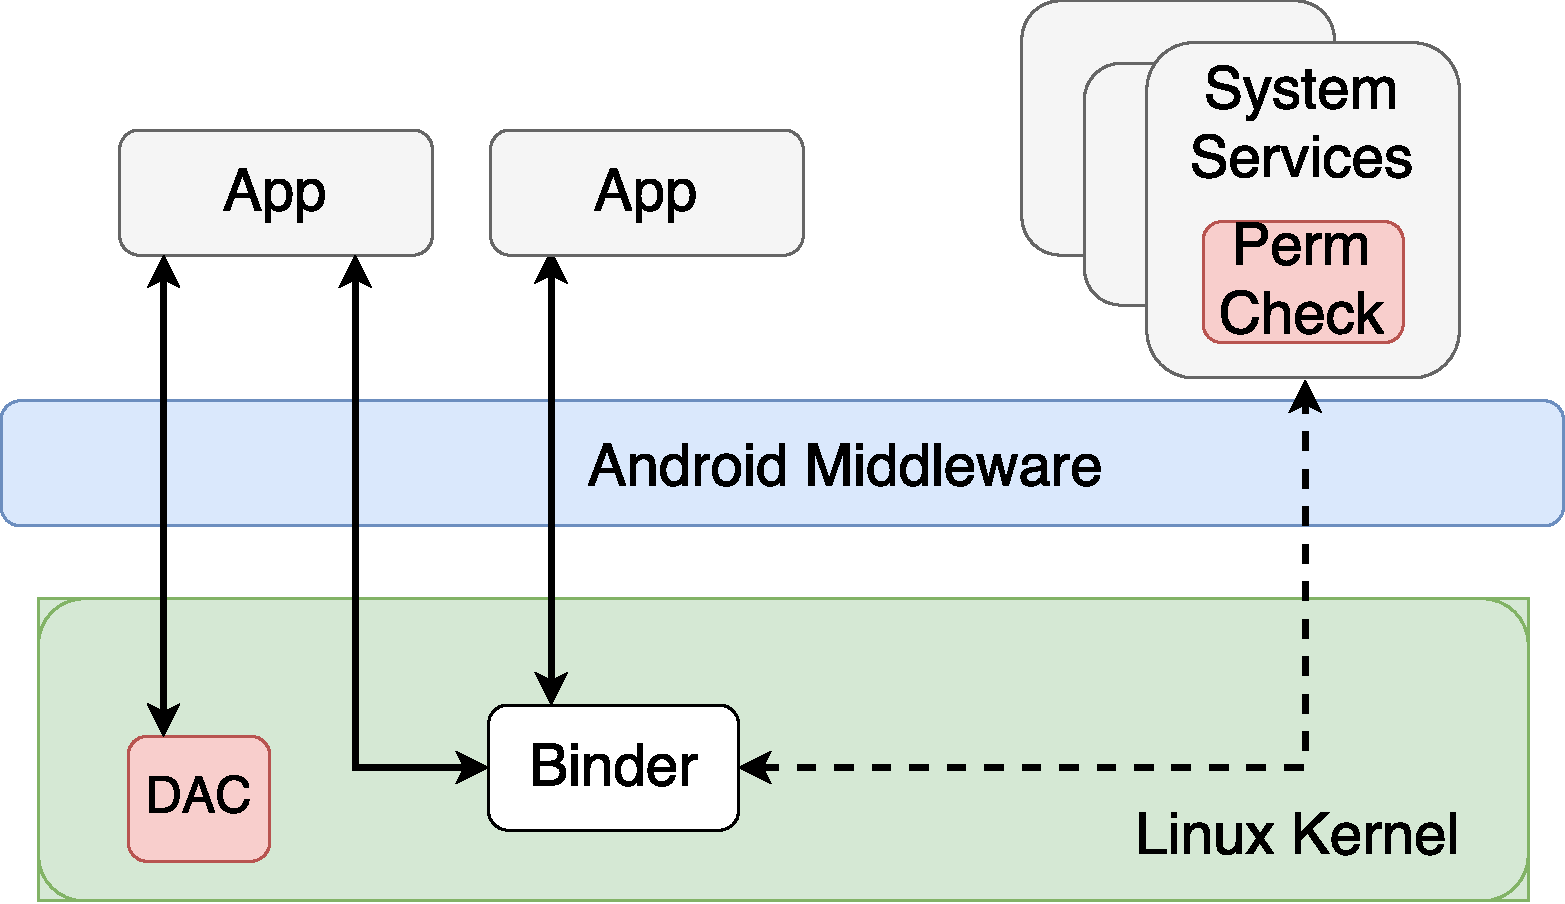
\includegraphics[width=.5\textwidth, keepaspectratio, resolution=600]{android_model}
\caption{Android Security model}
\label{fig:androidmodel}
\end{figure}


%-------Uncomment later.....
\iffalse
\begin{figure*}[!h]
\subfigure[Android execution model]{
\centering
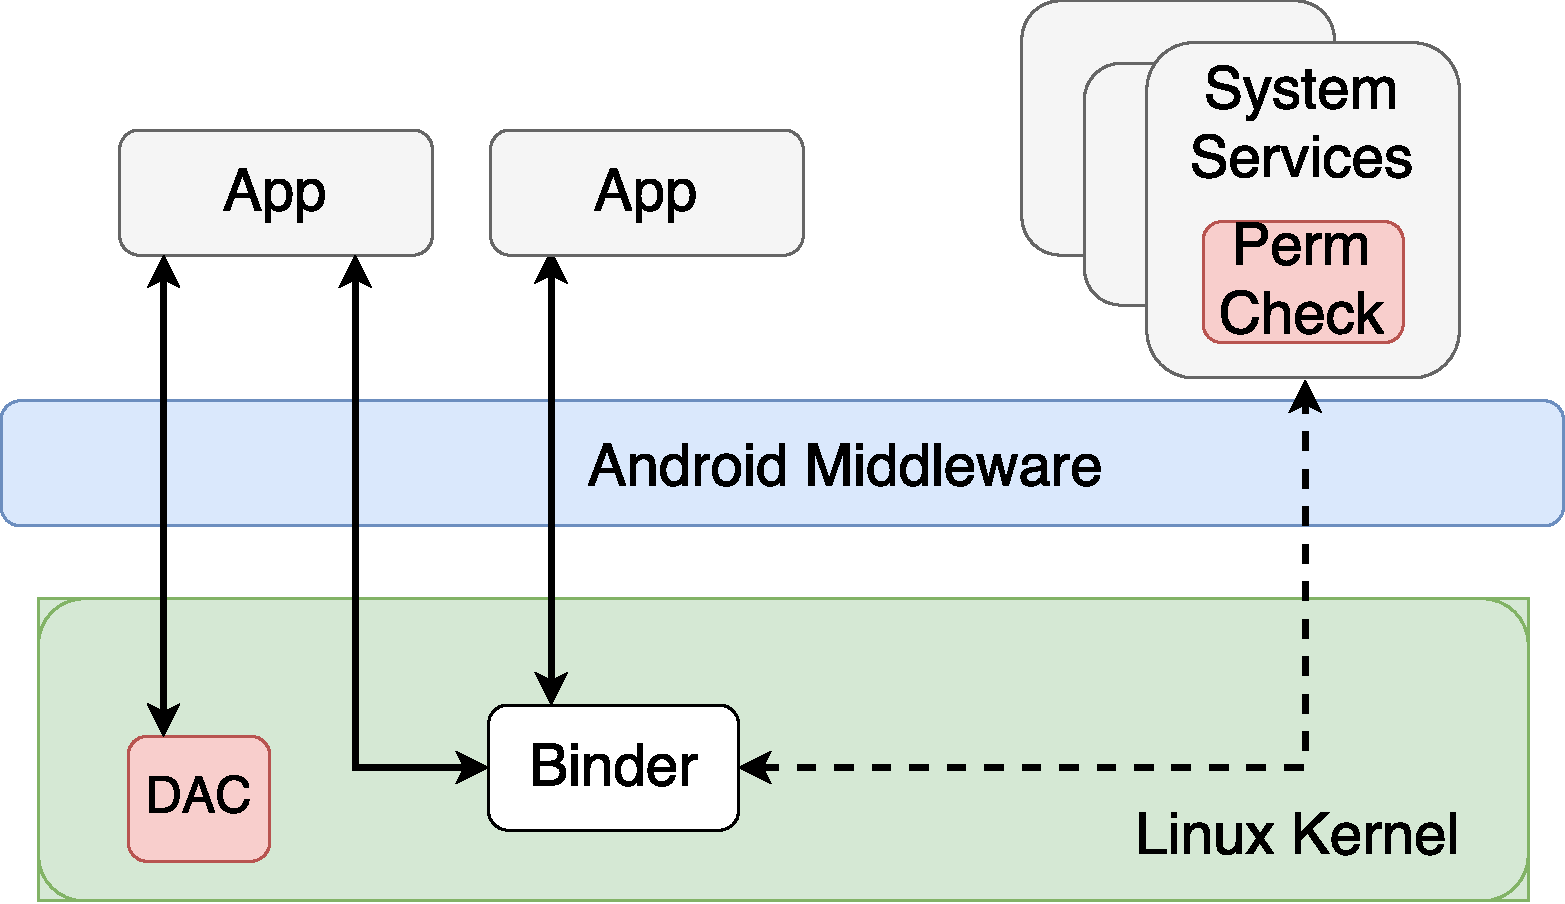
\includegraphics[width=.47\textwidth, keepaspectratio, resolution=600]{android_model}
\label{fig:sandbox-creation}
}
~%Nothing
\subfigure[\asd execution design]{
\centering
\includegraphics[width=.47\textwidth, keepaspectratio, resolution=600]{lightbox_model}
\label{fig:design}
}
\caption{LightBox (a) On-Device , (b) Sandbox Service}
\label{fig:lightbox}
\end{figure*}
\fi
%--------------------------


\textbf{Apps certificate.}  Android requires  all APKs to be digitally signed with a certificate. A public-key certificate contains the public key of a public/private key pair, as well as some other metadata identifying the owner of the key. The owner of the certificate holds the corresponding private key. When a developer signs an APK, the signing tool attaches the public-key certificate to the produced APK. The public-key certificate serves as a fingerprint that uniquely associates the APK to its developer and his corresponding private key. This helps Android to ensure that any future updates to that APK  come from the original developer. In fact, developers must use the same certificate throughout the lifespan of their apps to push new versions of their apps to the users' devices. In Android, a certificate authority is not mandatory: typically the app certificates do not need to be signed by a certificate authority and most developers use self-signed certificates.

\textbf{Android Manifest.} Android apps require to define a special file called \texttt{AndroidManifest.xml}, known as manifest\cite{manifest}, that contains specific meaningful information about the related Android app. Every app must have a manifest file in its root directory because the Android system needs to access its content before it can run any of the app's code. As a consequence, the manifest file cannot be obfuscated. The information declared in the manifest  cannot be changed at runtime: even  dynamically loaded code must comply with the permissions and the components defined in the app's manifest.

\textbf{Android \texttt{sharedUserId} attribute.} The manifest attribute \\ \shared, introduced since the first Android version, is a feature that allows to execute different apps under the same UID if and only if they are signed with the same certificate. Once installed, apps that share the same UID will have access to each other private data because they share the same Linux permissions set. This feature is extensively used by Android for core framework services and system apps. For instance, the Play Service and the Google location service use the \shared to request to run in the same process of the login service to be able to sync data in the background, without  user interaction. This feature is available to and widely used also by third-party developers to update their apps and shared libraries. Removing such features will have  an important impact on backward compatibility.
  
\textbf{Android \texttt{process} attribute.} The attribute \proc allows to execute two different apps within the same process space. It can be specified for any components in an app. Whenever the execution of  a component is requested, Android first looks for a running process matching the name specified in \proc. If a process is found, then that process will be used to execute the requested component. This avoids spawning a new process for a component if there is already a running instance of that component. For instance, this is used to reuse the background activity's process when it is called in foreground again.